\documentclass[%
 reprint,
%superscriptaddress,
%groupedaddress,
%unsortedaddress,
%runinaddress,
%frontmatterverbose, 
%preprint,
%showpacs,preprintnumbers,
%nofootinbib,
%nobibnotes,
%bibnotes,
 amsmath,
 amssymb,
 aps,
 pra,
%prb,
%rmp,
%prstab,
%prstper,
%floatfix,
 showkeys
]{revtex4-1}

\usepackage[utf8]{inputenc} 
\usepackage{colortbl}
\usepackage{graphicx}
\usepackage{hyperref}
\usepackage{ulem}

%\usepackage{epstopdf}

\usepackage{feynmp}
\DeclareGraphicsRule{*}{mps}{*}{}

\makeatletter
\def\endfmffile{%
  \fmfcmd{\p@rcent\space the end.^^J%
          end.^^J%
          endinput;}%
  \if@fmfio
    \immediate\closeout\@outfmf
  \fi
  \ifnum\pdfshellescape=\@ne
    \immediate\write18{mpost \thefmffile}%
  \fi}
\makeatother

\begin{document}


% Use the \preprint command to place your local institutional report
% number in the upper righthand corner of the title page in preprint mode.
% Multiple \preprint commands are allowed.
% Use the 'preprintnumbers' class option to override journal defaults
% to display numbers if necessary
%\preprint{}

%Title of paper
\title{Vector Boson Fusion Higgs Analysis in the Compact Muon Solenoid Experiment}

% repeat the \author .. \affiliation  etc. as needed
% \email, \thanks, \homepage, \altaffiliation all apply to the current
% author. Explanatory text should go in the []'s, actual e-mail
% address or url should go in the {}'s for \email and \homepage.
% Please use the appropriate macro foreach each type of information

% \affiliation command applies to all authors since the last
% \affiliation command. The \affiliation command should follow the
% other information
% \affiliation can be followed by \email, \homepage, \thanks as well.
\author{João Pela}
%\email[]{Your e-mail address}
%\homepage[]{Your web page}
%\thanks{}
%\altaffiliation{}
\affiliation{Imperial College London}

%Collaboration name if desired (requires use of superscriptaddress
%option in \documentclass). \noaffiliation is required (may also be
%used with the \author command).
%\collaboration can be followed by \email, \homepage, \thanks as well.
%\collaboration{}
%\noaffiliation

\date{\today}

\begin{abstract}
This is the 3 Month Report on my PhD Progress. Theoretical and experimental motivations for a Vector Boson Fusion 
Standard Model Higgs Search are presented at the Compact Muon Solenoid Experiment and the plans for future
analysis. A summary of the work already done on determining a working point for an invisible VBF Higgs Level 
1 Trigger and the ongoing work on an inclusive VBF trigger are summarized. This results have been presented 
to the CMS Collaboration and will be used for 2012 data taking. 
\end{abstract}

% insert suggested PACS numbers in braces on next line
%\pacs{}
% insert suggested keywords - APS authors don't need to do this
\keywords{High Energy Physics Experimental, Trigger Systems and Data Acquisition}

%\maketitle must follow title, authors, abstract, \pacs, and \keywords
\maketitle

\setlength{\unitlength}{1mm}

\section{Introduction and Motivation}

\subsection{Introduction}

The current knowledge on the field of particle physics is summarized in the Standard Model (SM). It is known that this model
is incomplete without the inclusion of a spontaneous symmetry breaking mechanism that would explain the observation 
that the electroweak bosons (the W and Z particles) have mass. The easiest way to introduce such a mechanism is
with the Higgs Mechanism, which suggests the presence of new yet to be observed particle, the Higgs Boson.

After 2 years of successful operation the experiments built on the Large Hadron Collider (LHC) at 
European Organization for Nuclear Research (CERN) located near Geneva, Switzerland were already able 
to further narrow down the possible mass range allowed experimentally for a Standard Model like Higgs Boson. 
The CMS collaboration has excluded at a 95\% confidence level the range 127-600 $GeV$. 
Some hits of a possible signal have already been seen around 124 $GeV$ with a significance of 1.5$\sigma$ 
(after look-elsewhere effect) but yet lack enough statistics to claim discovery
\cite{article:CMS-HIG-11-032}. Also, the ATLAS Collaboration have exclude at a 95\% confidence level the mass
ranges of 112.9–115.5 $GeV$, 131–238 $GeV$ and 251–466 $GeV$ and seen an excess of events around 126 $GeV$
with a significance of 2.2$\sigma$ (after look-elsewhere effect)\cite{article:CERN-PH-EP-2012-019}.
 
With the running condition targeted for the year 2012 at the LHC, physicists are confident that enough data will be
taken to discover or exclude a Standard Model Higgs.

\subsection{Higgs Phenomenology}

The main processes for Standard Model Higgs production are summarized at table \ref{table_HiggsDiagrams}.

\begin{table}[!ht]
\begin{tabular}{cc} 
\begin{fmffile}{feynmanDiagram_GFHiggs}
  \fmfframe(0,5)(0,5){
  \begin{fmfgraph*}(30,20)
    \fmfleft{g1,g2} \fmfright{H'}
    \fmf{gluon}{g1,t1}
    \fmf{gluon}{g2,t2}
    \fmf{fermion,tension=0,label=$t$,label.side=left}{t1,t2}
    \fmf{fermion,label=$t$,label.side=left}{t2,H}
    \fmf{fermion,label=$\bar{t}$}{H,t1}
    \fmf{boson}{H,H'}
    \fmflabel{$H^0$}{H'}
    \fmflabel{$g_1$}{g1}
    \fmflabel{$g_2$}{g2}
  \end{fmfgraph*}
  }
\end{fmffile}

(1) &

\begin{fmffile}{feynmanDiagram_VBFHiggs}
  \fmfframe(0,5)(0,5){
  \begin{fmfgraph*}(30,20)
    \fmfleft{P1,P2} \fmfright{P1',H',P2'}
    \fmf{fermion}{P1,g1}
    \fmf{fermion}{P2,g2}
    \fmf{boson,label=$W/Z^0$,label.side=left}{g1,H}
    \fmf{boson,label=$W/Z^0$,label.side=left}{H,g2}
    \fmfdot{H,g1,g1}
    \fmf{boson,tension=0.2}{H,H'}
    \fmf{fermion}{g1,P1'}
    \fmf{fermion}{g2,P2'}
    \fmflabel{$H^0$}{H'}
    \fmflabel{$q_1$}{P1}
    \fmflabel{$q_2$}{P2}
    \fmflabel{$q_1'$}{P1'}
    \fmflabel{$q_2'$}{P2'}
  \end{fmfgraph*}
  }
\end{fmffile}
(2) \\
\begin{fmffile}{feynmanDiagram_ttFHiggs}
  \fmfframe(0,5)(0,5){
  \begin{fmfgraph*}(30,20)
    \fmfleft{g2,g1} 
    \fmfright{t2',H',t1'}
    \fmf{gluon}{g2,t2}
    \fmf{gluon}{g1,t1}
    \fmf{fermion}{t2',t2}
    \fmf{fermion,label.side=right,label=$t$}{t2,H}
    \fmf{fermion,label.side=right,label=$\bar{t}$}{H,t1}
    \fmf{fermion}{t1,t1'}
    \fmf{boson,tension=0.5}{H,H'}
    \fmflabel{$H^0$}{H'}
    \fmflabel{$g_1$}{g1}
    \fmflabel{$g_2$}{g2}
    \fmflabel{$t$}{t1'}
    \fmflabel{$\bar{t}$}{t2'}
  \end{fmfgraph*}
  }
\end{fmffile}
(3) &

\begin{fmffile}{feynmanDiagram_WZstrahlung}
  \fmfframe(0,5)(0,5){
  \begin{fmfgraph*}(30,20)
    \fmfleft{q2,q1} \fmfright{H',V'}
    \fmf{fermion}{v1,q2}
    \fmf{fermion}{q1,v1}
    \fmf{boson,label=$W/Z$}{v1,v2}
    \fmf{boson}{v2,V'}
    \fmf{boson}{v2,H'}
    \fmflabel{$H^0$}{H'}
    \fmflabel{$W/Z$}{V'}
    \fmflabel{$q$}{q1}
    \fmflabel{$\bar{q}$}{q2}
  \end{fmfgraph*}
  }
\end{fmffile}
(4)

\end{tabular}
\label{table_HiggsDiagrams}
\caption{Main processes for Standard Model Higgs production ordered by highest cross section at the LHC. (1) Gluon Fusion, 
(2) Vector Boson Fusion, (3) $t\bar{t}$ Fusion and (4) $W/Z$ associated production.}
\end{table}

The respective cross sections for each production process can be found in figure \ref{figure_SMHiggs_XSec}
\cite{Takahashi:1019873}. It can be seen that the Gluon Fusion (GF) is the leading process by almost one order of magnitude higher than Vector 
Boson Fusion (VBF) which is the second most frequent process in the currently allowed experimental mass range for a 
Standard Model Higgs Boson. Both $t\bar{t}$ Fusion and Weak Boson associated productions have cross sections more than
one order of magnitude lower than VBF in the same mass range.

\begin{figure}[ht]
\centering
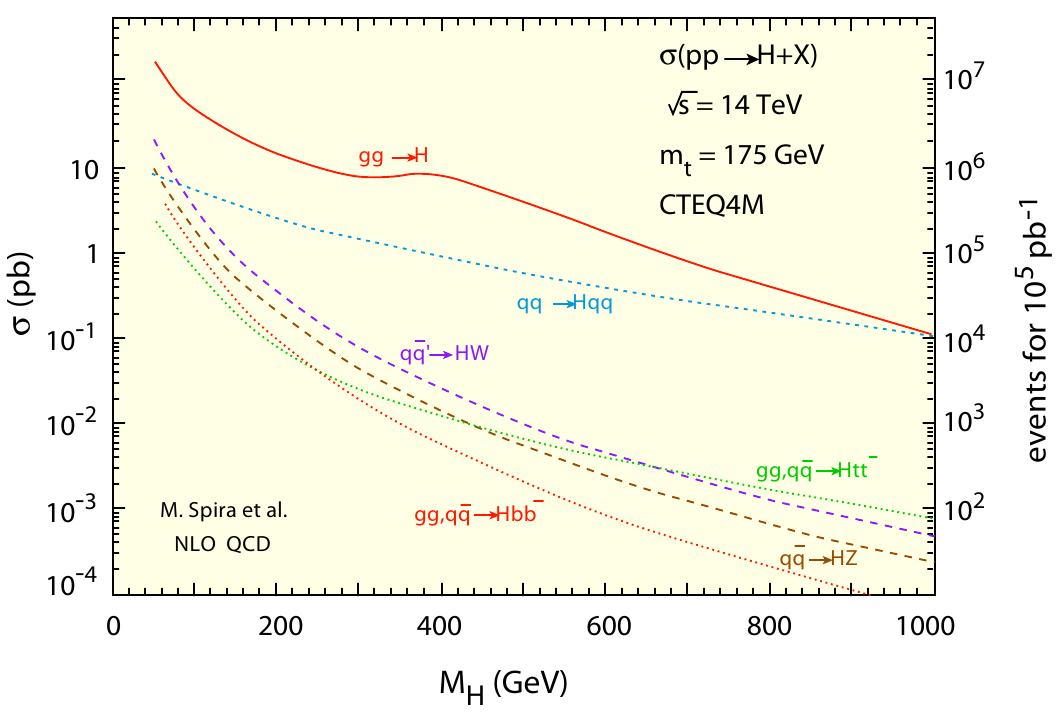
\includegraphics[width=0.45\textwidth]{img/SMHiggs_XSec.png} 
\caption{Theoretical prediction of Standard Model Higgs productions cross sections for a $\sqrt(s)=14$ $TeV$ 
and assuming $m_{top}=175$ $GeV$.}
\label{figure_SMHiggs_XSec}
\end{figure}

The Higgs Boson will than decay with different probabilities to different objects depending on its mass, a plot
of this probabilities can be found at figure \ref{figure_SMHiggs_BR} \cite{Takahashi:1019873}. We can see that the 
allowed decay channels for the non-excluded experimental mass range are by order of likeliness $b\bar{b}$, 
$\tau\bar{\tau}$, $c\bar{c}$, $gg$, $\gamma\gamma$ and $Z\gamma$.

\begin{figure}[ht]
\centering
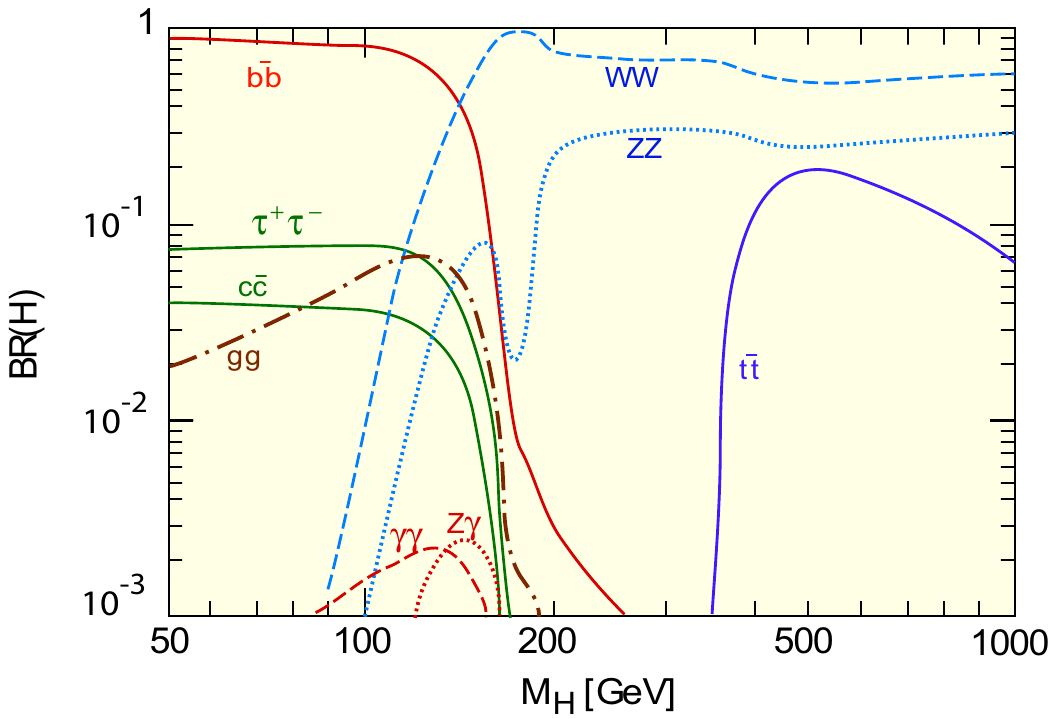
\includegraphics[width=0.45\textwidth]{img/SMHiggs_BR.png} 
\caption{Theoretical prediction of Standard Model Higgs branching rations as a function of its mass.}
\label{figure_SMHiggs_BR}
\end{figure}

\subsection{Motivation}

The first theoretical motivations for looking for VBF Higgs events is obviously to observe and measure its
cross section and each of the branching ratios for its decays. We can then calculate its coupling to the 
Week Bosons and to fermions (including the leptonic sector via $\tau\bar{\tau}$). From the couplings we may be able to
differentiate between a SM Higgs or Beyond the Standard Model (BSM) Higgs like one of the Super Symmetric
incarnations of this boson\cite{article:Duhrssen:2004cv,article:Zeppenfeld:2000td}. And, if the Higgs will only decay invisibly like it is predicted by Higgs Fermiophobic 
Models, VBF is the primary discovery channel.

From the experimental point of view, we can see from figure \ref{figure_SMHiggs_XSec} that VBF has a cross section
one order of magnitude lower than GF, but we should notice from diagram 2 in table \ref{table_HiggsDiagrams} that
there are two forward jets produced along with the Higgs and we can use them for tagging. Also we can profit from
the lack of colour exchange between the interacting quarks which will result in low hadronic activity in the 
central rapidity region. Since the Higgs visible decay products (if any) are most likely produced in the 
central rapidity region, this means that they will be likely isolated from the forward jets thus allowing better 
reconstruction/identification efficiency which should allow easier study of the Higgs properties.

\section{The Large Hadron Collider}

The Large Hadron Collider (LHC) is at this moment the world's largest and highest-energy particle accelerator
in activity. It was built in a 27 kilometer circular tunnel, at an average depth of around 100 meters, under the
Franco-Swiss border near Geneva, Switzerland\cite{Bruning:2004ej}.

The LHC is a synchrotron machine designed to accelerate and collide two opposing particle beams of particles.
Particles are injected into the machine in bunches, which can be composed of protons or lead nuclei. For
protons the maximum nominal energy that can be achieved per beam is 7 $TeV$, which represents 14 $TeV$ in the 
center of mass frame for a single proton-proton collision. While for lead nuclei a maximum nominal energy of 
574 $TeV$ per nucleus (2.76 $TeV$ per nucleon) per beam is planned. The running conditions for proton collisions
during 2012 are predicted to be 8 $TeV$ center of mass energy, with initially an average number pile up collisions
of the order of 28 and a delivering instant luminosity of the order of $5 \times 10^{33}$ $cm^{-2}s^{-2}$

\section{The Compact Muon Solenoid Experiment}

The Compact Muon Solenoid Experiment (CMS) is a general purpose experiment that is an integrating part of the LHC
program. It was designed to study the collisions of two intersecting proton beams in its center \cite{article:CMSTDRv12006}. 
This detector was planned with the intention of studying a broad spectrum of physics processes and is made of several
subsystems, each one designed to take advantage of some characteristics of the particles produced in order to
measure their energy, momentum and charge. The detector has classical onion structure with several layers, starting
from the collision point outwards we have: Tracker System, Electromagnetic Calorimeter, Hadronic Calorimeter,
Magnet, Muon System and Return Yoke.

At nominal conditions forty million collisions are produced in a single second and it would be impossible to 
register all of them. As collisions are uninteresting, the solution is having some kind of event selection 
already in the machine so we would only save the most interesting collisions. This is the role of the Trigger System, 
which over two levels (each one with more information of what happened), reduces the number of events to a 
manageable rate.

The overall dimensions of CMS detector are a length of 21.6 $m$, a diameter of 14,6 $m$, and total weight of 
12500 $tons$.

\section{VBF Signature at CMS}

The Standard Model Higgs Vector Boson Fusion (VBF) signature main characteristic is the presence of two forward jets
associated with the Higgs (see diagram 2 in table \ref{table_HiggsDiagrams}). This two forward jets have a reasonable 
$p_T$ ($\gtrsim30$ $GeV$), high $\Delta\eta$ separation between them ($\gtrsim 3)$ and low $\Delta\phi$ ($\lesssim 2.5$). 
The dijet pair also has a high invariant mass since it will be produced back-to-back to the Higgs Boson. Because there 
is no color exchange between the incoming quarks the hadronic activity between the jets is suppressed. On the other 
hand the Higgs decay products if any will be located at the central rapidity area which will be easier to study because of the low hadronic activity
already described\cite{article:Dokshitzer:1991he}. The distribution of the pseudo-rapidity for both forward jets and two $\tau$ coming form SM Higgs
decay of simulated events at the CMS detector can be found in \ref{figure_VBF_HToTauTau_ObjectsRapidityGap}.

\begin{figure}[ht]
\centering
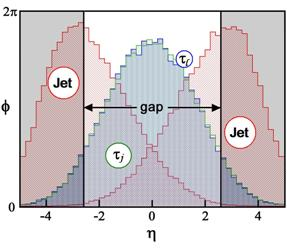
\includegraphics[width=0.45\textwidth]{img/ObjectsRapidityGap.jpeg} 
\caption{Simultaneous plot of the $\eta$ coordinate of both forward jets and the $\tau\bar{\tau}$
produced from simulated VBF Higgs decay. Super-imposed with 4 circle showing the possible positions of this 4
object in an hypothetical event.}
\label{figure_VBF_HToTauTau_ObjectsRapidityGap}
\end{figure}

The CMS detector is ideal for this type of searches since it is an $4\pi$ hermetic detector with calorimeter coverage
from -5 to 5 in pseudo-rapidity, it also has very good capabilities of particle measurement and identification which can be used
to identify the forward jets and Higgs decay products or in case of an invisible decay, compute the resulting missing 
transverse energy. An event display of a simulated Standard Model Higgs (which than decays to $\tau\bar{\tau}$) produced 
via VBF can be found at figure \ref{figure_EventDisplay_VBF_HToTauTau_El-Had}.

\begin{figure}[ht]
\centering
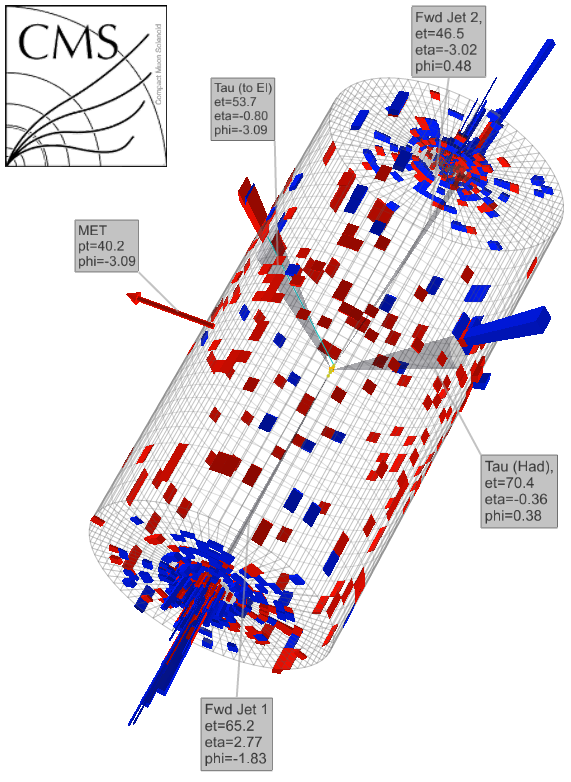
\includegraphics[width=0.45\textwidth]{img/EventDisplay_VBF_HToTauTau_El-Had.png} 
\caption{Event display of a simulated event where a Standard Model Higgs is produced via Vector Boson Fusion
which than decays to $\tau\bar{\tau}$ which in turn decay leptonically to electron (left) and hadronically (right).}
\label{figure_EventDisplay_VBF_HToTauTau_El-Had}
\end{figure}

\section{L1 Trigger Studies}

\subsection{Invisible Higgs Trigger}

I have been involved in a study of a CMS Level 1 Trigger algorithm with the objective of efficiently selecting
VBF Higgs to invisible decays. This study was based on real data from the High Pileup special run taken late 2012
and was aimed at making a proposal for a viable trigger algorithm to be used in the 2011 proton run.

The algorithm was based on selecting missing transverse energy (MET) and two jets that would pass the test 
$\eta_{jet1}\times\eta_{jet2}<0$ and would have a separation of $\Delta\eta_{jj}>3$. An possible additional cut
was also studied, a restriction on $\Delta\phi_{jj}$, tested points were no cut, $<2.5$, $<2.1$ and $<1.8$. For the
conditions expected on early 2012 (i.e. instant luminosity of $5e33$ and $<PU>=28$) two tables were produced
reporting the cuts necessary to achieve a give rate threshold,
one assuming fixed dijet $E_\bot$ cut and varying MET (table \ref{table_5E33_PU28_fixedDijet}) and another
assuming fixed MET cut and varying $E_\bot$ (table \ref{table_5E33_PU28_fixedMET}). 

\begin{table} 
\begin{tabular}{|c||c|c|c|c|}
\hline
\multicolumn{5}{|c|}{MET [GeV] ($E_\bot(jj)>20$ [GeV])} \\
\hline
$\Delta\phi$ & no cut & 2.5 & 2.1 & 1.8 \\
\hline
10kHz        &     32 &  32 &  32 &  32 \\
5kHz         &     35 &  35 &  35 &  35 \\
\cellcolor{green}2kHz &\cellcolor{green}      41 &  41 &  41 &  41 \\
1kHz         &     47 &  47 &  47 &  46 \\
500Hz        &     54 &  54 &  54 &  53 \\
\hline
\end{tabular}
\caption{Cut thresholds to apply to MET assuming fixed dijet $E_\bot>20$ [GeV] to obtain specif L1 Rates forced
instant luminosity of $5e33$ and $<PU>=28$. Highlighted in green is the working point suggested to the Tigger 
Studies Group for the L1 Trigger.}
\label{table_5E33_PU28_fixedDijet}
\end{table}

\begin{table} 
\begin{tabular}{|c||c|c|c|c|}
\hline
\multicolumn{5}{|c|}{$E_\bot(jj)$ [GeV] ($MET>30$ [GeV])} \\
\hline
$\Delta\phi$ & no cut & 2.5 & 2.1 & 1.8 \\
\hline
10kHz        &     28 &  28 &  24 &  24 \\
5kHz         &     32 &  32 &  32 &  32 \\
\cellcolor{green} 2kHz         &\cellcolor{green}      52 &  48 &  44 &  44 \\
1kHz         &     68 &  68 &  64 &  64 \\
500Hz        &     92 &  92 &  88 &  88 \\
\hline
\end{tabular}
\caption{Cut thresholds to apply to dijet $E_\bot$ assuming fixed dijet $MET>30$ [GeV] to obtain specif L1 Rates forced
instant luminosity of $5e33$ and $<PU>=28$. Highlighted in green is the working point suggested to the Tigger 
Studies Group for the L1 Trigger.}
\label{table_5E33_PU28_fixedMET}
\end{table}

Results were used to define working points for this trigger, which were already proposed to the Trigger Studies Group
to be included on a future L1 Trigger Menus. Proposed trigger were:
\begin{itemize}
  \item Dijet $E_\bot>20$ $GeV$ + fwd/bkwd + $\Delta\eta_{jj}>3$ + $MET>40$ $GeV$
  \item Dijet $E_\bot>50$ $GeV$ + fwd/bkwd + $\Delta\eta_{jj}>3$ + $MET>30$ $GeV$
\end{itemize}

Further studies were made for conditions predicted for late 2012 (i.e. instant luminosity of $7e33$ and $<PU>=32$)
and can be found on tables \ref{table_7E33_PU32_fixedDijet} and \ref{table_7E33_PU32_fixedMET}.

\begin{table} 
\begin{tabular}{|c||c|c|c|c|}
\hline
\multicolumn{5}{|c|}{MET [GeV] ($p_\bot(jj)>20$ [GeV])} \\
\hline
$\Delta\phi$ & no cut & 2.5 & 2.1 & 1.8 \\
\hline
10kHz        &     36 &  36 &  36 &  36 \\
5kHz         &     40 &  40 &  40 &  40 \\
2kHz         &     47 &  47 &  47 &  46 \\
1kHz         &     54 &  54 &  54 &  54 \\
500Hz        &     67 &  66 &  66 &  64 \\
\hline
\end{tabular}
\caption{Cut thresholds to apply to MET assuming fixed dijet $E_\bot>20$ [GeV] to obtain specif L1 Rates forced
instant luminosity of $7e33$ and $<PU>=32$}
\label{table_7E33_PU32_fixedDijet}
\end{table}

\begin{table} 
\begin{tabular}{|c||c|c|c|c|}
\hline
\multicolumn{5}{|c|}{$p_\bot(jj)$ [GeV] ($MET>30$ [GeV])} \\
\hline
$\Delta\phi$ & no cut & 2.5 & 2.1 & 1.8 \\
\hline
10kHz        &     32 &  32 &  32 &  32 \\
5kHz         &     40 &  40 &  40 &  40 \\
2kHz         &     64 &  60 &  60 &  56 \\
1kHz         &     76 &  76 &  76 &  76 \\
500Hz        &    100 & 100 &  96 &  92 \\
\hline
\end{tabular}
\caption{Cut thresholds to apply to dijet $E_\bot$ assuming fixed dijet $MET>30$ [GeV] to obtain specif L1 Rates forced
instant luminosity of $7e33$ and $<PU>=32$}
\label{table_7E33_PU32_fixedMET}
\end{table}

\subsection{Inclusive Higgs Trigger}

It would be desirable to have a dedicated inclusive L1 Trigger (i.e. Higgs decay independent). Such a trigger
would allow to have a single trigger for all VBF signature analysis, which implies less systematics 
while comparing them and usually the more people using a trigger means it will become better understood by all.
 
By triggering only on the VBF signature we therefore have no dependence on the Higgs decay, which means
we can get all possible decays with a single trigger, even those that are predicted by yet to be defined models.
Thus, it would be a model independent trigger.

If it happens that we do not find any Higgs boson, this trigger can than be used for a WW scattering analysis, aimed 
at Standard Model exclusion, since the signature is similar.

For such a trigger to work it would have to be based only on the forward dijet present on the VBF signature. 
It was decided to study three variables: Invariant Mass, Transverse Invariant Mass (MT) and Scalar Sum of the 
Hadronic Energy (HT). Again, we always require a dijet with $\Delta\eta>3$ and we study the effects of an additional cut
on $\Delta\phi$, the points tested were no cut, $<2.5$, $<2.1$ and $<1.8$).
  
\subsubsection{Invariant Mass}

This variable takes advantage from the very high invariant mass of the dijet system but it is not yet implemented 
on the L1 Hardware but it is in principle possible.

Unfortunately this variable was showed to be unusable. To get acceptable rates we would need to cut too high on 
Jet $p_\bot$ or $M_{Inv}$ losing almost all signal efficiency.

\subsubsection{Transverse Invariant Mass}

This variable is better at suppressing QCD events, it is less pileup dependent and has lower error associated to it
(only x-y dependence). It is also not yet implemented on the L1 Hardware but should also be possible to develop. 

This variable showed to be promising. A possible working point for a Level 1 rate 
of 5kHz could be $MT>50$ $GeV$ no $\Delta\phi$ cut and dijet $p_\bot \sim 45$ $GeV$ which should give a signal 
efficiency of $\lesssim70\%$ (see R. Lane 3 Months PhD Report).

\subsubsection{HT (Scaler Sum of the Transverse Energy)}

Theoretically this is the best variable to separate signal from background and has the advantage of being already 
implemented on L1 Hardware.

This was showed to be the most promising variable. A possible working point for a Level 1 rate of 5kHz could be $HT>100$ $GeV$ no 
$\Delta\phi$ cut and dijet $p_\bot \sim 40$ $GeV$ which should give a signal efficiency of $\lesssim98\%$ 
(see R. Lane talk, \ref{figure_PU28_5e33_RateFBDijetDEtaDPhi00HT100} and \ref{figure_sig_eff_l1_ht}).

\begin{figure}[ht]
\centering
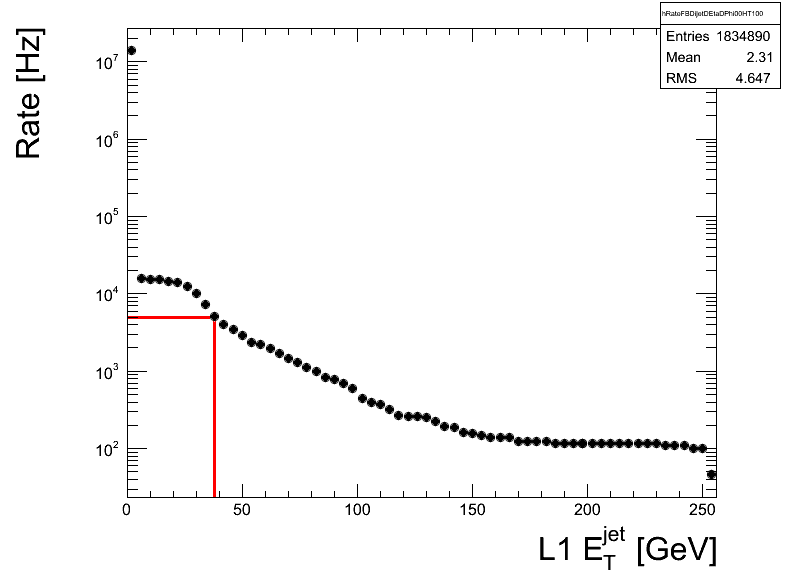
\includegraphics[width=0.45\textwidth]{img/PU28_5e33_RateFBDijetDEtaDPhi00HT100.png} 
\caption{Level 1 rate as a function of dijet $p_\bot$ while selecting events with $HT>100$ $GeV$. Results based on
date from the High Pileup Special run taken late 2011.}
\label{figure_PU28_5e33_RateFBDijetDEtaDPhi00HT100}
\end{figure}

\begin{figure}[ht]
\centering
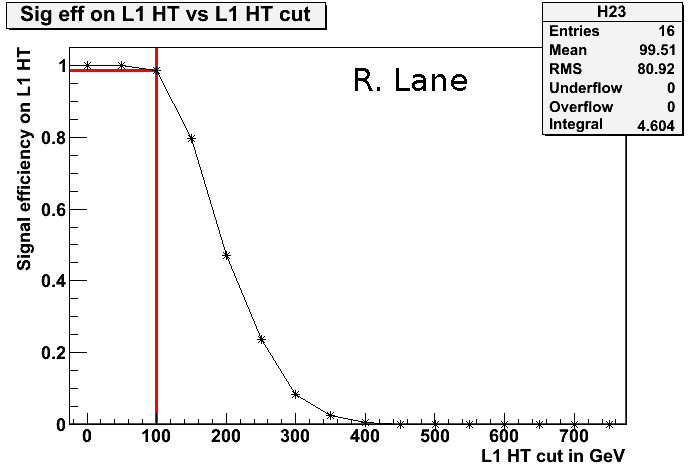
\includegraphics[width=0.45\textwidth]{img/sig_eff_l1_ht.png} 
\caption{Higgs to $\tau\bar{\tau}$ signal efficiency as a function of HT cut extracted from monte carlo simulation.
Result from R. Lane.}
\label{figure_sig_eff_l1_ht}
\end{figure}
  
\section{Plans}

My plans are, to participate on the L1-HLT inclusive VBF Trigger development, commissioning and maintenance.   
This trigger will be the basis of a data analysis of a VBF Higgs decay channel, which on a first stage will aim at 
observation and later at properties measurement.

In parallel I will participate on trigger related efforts like, Data Quality Monitoring (DQM), trigger upgrades 
development and other types of service work.

\section{Conclusions}

There will be a VBF Higgs to Invisible dedicated trigger for 2012. Most likely an inclusive VBF trigger will be 
included soon, which should cover most of the 2012 data. The year of 2012 will be an exciting year for all the LHC 
experiments, where we may finally find hits of new physics and/or be forced the rethink our current knowledge of
particle physics. 
 
Imperial College CMS Group highly involved on the trigger efforts for a VBF analysis. This will evolve quickly 
with data to a full analysis effort aimed at publication of the (soon to be discovered) Higgs Boson properties.

\bibliographystyle{abbrv}
\bibliography{JPela_PhDReport3M_Bibliography}

\end{document}